\documentclass{beamer}

\usepackage[utf8]{inputenc}
\usepackage[russian]{babel}
\usepackage{hyperref}
\usepackage{graphicx}
\usepackage{listings}
\usepackage{ucs}

\lstset{
    extendedchars=\true,
    inputencoding=utf8x
}

\usetheme{Warsaw}
\usecolortheme{lily}
\useoutertheme[subsection=false]{smoothbars}
\useinnertheme{circles}
\setbeamertemplate{footline}[page number]{}
\setbeamertemplate{navigation symbols}{}

\renewcommand{\figurename}{} 

\title{Архитектура ЭВМ}
\subtitle{Лекция 4. Чем удобны ЯП высокого уровня?}
\author{к.ф.-м.н. Филонов Павел Владимирович \\ filonovpv@gmail.com}
\date{22 сентября 2013 г.}


\institute[МГТУ ГА] 
{
    Московский Государственный Технический Университет \\
    Гражданской Авиации
}
\begin{document}
    \frame{\titlepage}
    \begin{frame}{Смотрите в этой серии}
        \begin{enumerate}
        \pause
        \item Типы данных и форматы констант
        \pause
        \item Арифметика на x86
        \pause
        \item Disassemble\&Debugging 
        \pause
        \item Jump'ов разных и побольше!
        \pause
        \item Логические операции
        \end{enumerate}
    \end{frame}
    \section{Ассемблер NASM}
    \subsection{}
    \begin{frame}[fragile]
        \frametitle{Структура программы}\small
        \begin{verbatim}
; NASM example program
; by Filonov Pavel (filonovpv at gmail.com)
; 23 Jul 2013

%include "stud_io.inc"

global _start

section .data ; секция инициализированных данных
    ; ...

section .bss  ; секция неинициализированных данных 
    ; ...

section .text ; секция исполняемого кода
_start:
    ; ...
    FINISH
        \end{verbatim}
\end{frame}
    \begin{frame}[fragile]
        \frametitle{DB и его друзья}\small
        \begin{verbatim}
;<метка> <псевдоинструкция> <список значений> 
ten dd 10 
msg db "Hello, world"\end{verbatim}
        \begin{block}{Псевдоинструкции в .data}\small
            \begin{verbatim}
db  0x55                 ; просто байт 0x55
db  0x55, 0x56, 0x57     ; три байта по порядку
db  'a', 0x55            ; можно использовать символы
db  'hello', 13, 10, '$' ; как и строки
dw  0x1234               ; 0x34 0x12
dw  'a'                  ; 0x61 0x00 (просто число)
dw  'ab'                 ; 0x61 0x62 (символьная константа)
dw  'abc'                ; 0x61 0x62 0x63 0x00 (строка)
dd  0x12345678           ; 0x78 0x56 0x34 0x12
dd  1.234567e20          ; число с плавающей точкой
dq  0x123456789abcdef0   ; 8-ми байтное число
dq  1.234567e20          ; число двойной точности
dt  1.234567e20          ; число увеличенной точности
            \end{verbatim}
        \end{block}
\end{frame}
    \begin{frame}[fragile]
        \frametitle{RESB и его друзья}\small
        \begin{verbatim}
;<метка> <псевдоинструкция> <размер> 
ten dd 10 
msg db "Hello, world"\end{verbatim}
        \begin{block}{Псевдоинструкции в .bss}
            \begin{verbatim}
buffer      resb    64  ; резервирует 64 байта
wordvar     resw    1   ; резервирует одно слово (2 байта)
regval      resd    1   ; размер одного регистра (4 байта)
realarray   resq    10  ; массив из 10 вещественных чисел\end{verbatim}
        \end{block}
        \begin{block}{EQU}
        \begin{verbatim}
msg db "Hello, world", 0x0a
len equ $-msg\end{verbatim}
        \end{block}
        \begin{block}{INCBIN}
        \begin{verbatim}
incbin "file.dat"          ; вставить весь файл
incbin "file.dat",1024,512 ; пропустить первые 1024 байта и
                           ; и вставить не больше 512 байт\end{verbatim}
        \end{block}
\end{frame}
    \begin{frame}[fragile]
        \frametitle{Числовые константы}
        \begin{verbatim}
200         ; десятичная
0200        ; всё ешё десятичная
0200d       ; явно десятичная
0d200       ; также десятичная
0c8h        ; шестнадцатиричная (hex)
$0c8        ; снова hex (0 обязательно)
0xc8        ; опять hex
0hc8        ; всё ещё hex
310q        ; восьмиричная
0o310       ; опять восьмиричная
0q310       ; и снова восьмиричная
11001000b   ; двоичная
1100_1000b  ; таже двоичная конста
1100_1000y  ; и снова двоичная
0b1100_1000 ; она же
0y1100_1000 ; всё ещё двоичная       
        \end{verbatim}
\end{frame}

    \section{Арифметика}
    \subsection{}
    \begin{frame}[fragile]
        \frametitle{Команда MOV}
        {\bf MOV} (Move) --- набор команд, предназначенных для пересылки данных из одного места в другое
        \begin{block}{Виды операндов}\small
        \begin{verbatim}
mov eax, ebx       ; из одного регистра в другой
mov eax, 112       ; задать(непосредственным операндом)
                   ; значение регистра
mov eax, [count]   ; из памяти в регистр, здесь
                   ; count - адрес в памяти (метка), а
                   ; [count] - значение по этому адресу
mov [count], eax   ; из регистра в память
mov [x], dword 25  ; задать(непосредственным операндом)
                   ; значение ячейки памяти\end{verbatim}
        \end{block}
        \begin{block}{Сцецификаторы размеров операнда}\footnotesize
        \begin{itemize}
            \item byte --- байт
            \item word --- слово (2 байта)
            \item dword --- двойное слово (4 байта)
        \end{itemize}
        \end{block}
\end{frame}
    \begin{frame}[fragile]
        \frametitle{Исполняемый адрес}
        \begin{figure}
        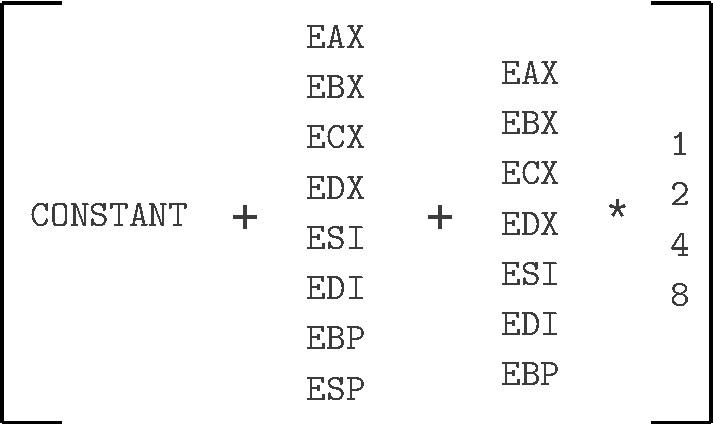
\includegraphics[width=0.7\linewidth]{fig/effective_addr.pdf}
        \end{figure}
        {\bf LEA} (Load Effective Address) --- загружает в регистр вычисленное значение исполняемого адреса. Обращение к памяти не производится
        \begin{verbatim}
lea edi, [array + eax + 4*ebx]
        \end{verbatim}
\end{frame}
    \begin{frame}{Пример}
    \end{frame}
    \begin{frame}[fragile]
        \frametitle{Команды сложения и вычитания}
        {\bf ADD} (Addition) --- целочисленное сложение

        {\bf SUB} (Substraction) --- целочисленное вычитание
        \begin{block}{Примеры}
            \begin{verbatim}
add eax, ebx        ; eax := eax + ebx
add al,  cl         ; al := al + cl
add al,  10         ; al := al + 10
sub ebx, [a]        ; ebx := ebx - [a] 
sub [a], dword 100  ; [a] := [a] - 100
            \end{verbatim}
        \end{block}
        Команды ADD и SUB устанавливают флаги (ZF, SF, OF, CF, PF)

        {\bf ADC} (Add with Carry) --- сложить с переносом (к сумме прибавляется значение флага CF)

        {\bf SBB} (Substraction with Borrow) --- вычитание с заимствованием (из разности вычитается CF)
\end{frame}
    \begin{frame}[fragile]
        \frametitle{Команды \tt inc, dec, neg и cmp}
        {\bf INC} (Increase) --- увеличивает значение операнда на единицу

        {\bf DEC} (Decrease) --- уменьшает значение операнда на единицу

        Команды INC, DEC устанавливают флаги ZF, OF, SF (но не CF)

        \bigskip
        {\bf NEG} (Negative) --- изменяет знак числа (вычисляет дополнительный код)

        {\bf CMP} (Compare) --- вычитает второй операнд из первого (результат не сохраняется). CMP используется ради установки флагов и обычно за ним следует условный переход
\end{frame}
    \begin{frame}[fragile]
        \frametitle{Целочисленное умножение и деление}
\end{frame}
\end{document}